% ffsp.tex
% Appendix section to describe how ffsp works
% Stephan Gahima/paper-draft-tex

\section{\texttt{ffsp} \label{sec:ffsp} - Examples}
	
	Please refer to the Matlab examples located in the \texttt{matlab/examples} folder. 
	The figures in \reffig{fig:2-by-3}, \reffig{fig:2-by-2}, and \reffig{fig:4-by-4} are generated from the following files: \texttt{complex\_2\_by\_3.m}, \texttt{matlab\_logo\_2\_by\_2.m}, and \texttt{tansin\_4\_by\_4.m}, respectively.
	
	\begin{figure}[H]
		\centering
		% matlab/examples/complex_2_by_3.m
		\begin{subfigure}[b]{\threefig\textwidth}
			\centering
			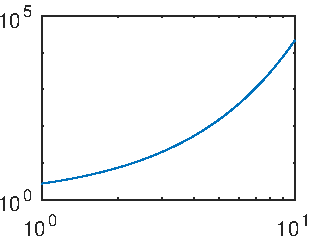
\includegraphics{../matlab/fig/examples/loglog-with-ffsp.pdf}
			\subcaption{Log plot.}
		\end{subfigure}
		\hfil
		\begin{subfigure}[b]{\threefig\textwidth}
			\centering
			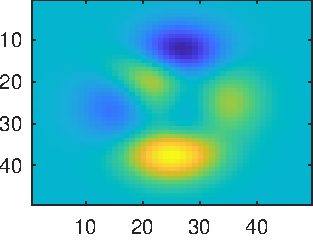
\includegraphics{../matlab/fig/examples/peaks-with-ffsp.pdf}
			\subcaption{Image from array.}
		\end{subfigure}
		\hfill
		\begin{subfigure}[b]{\threefig\textwidth}
			\centering
			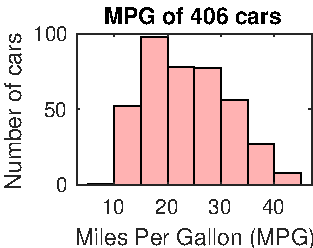
\includegraphics{../matlab/fig/examples/hist-with-ffsp.pdf}
			\subcaption{Histogram.}
		\end{subfigure}
		\\
		\begin{subfigure}[b]{\onefig\textwidth}
			\centering
			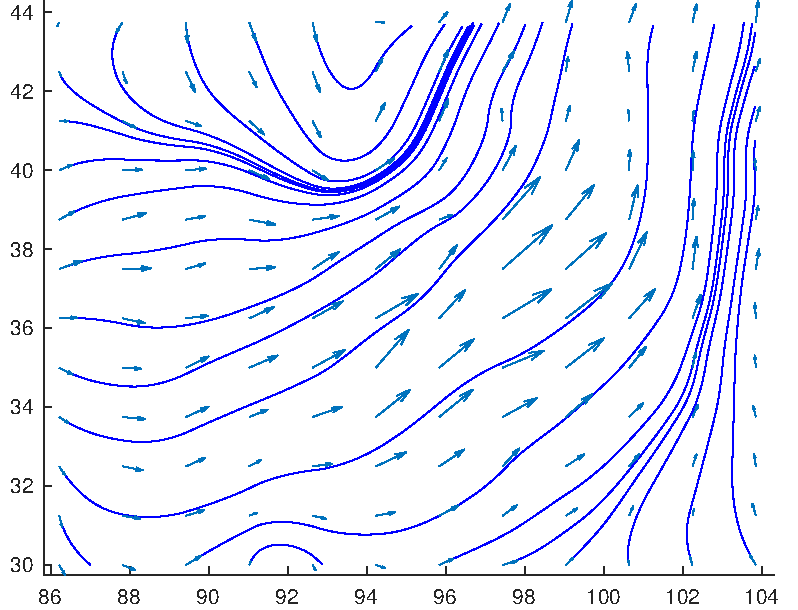
\includegraphics{../matlab/fig/examples/stream-with-ffsp.pdf}
			\subcaption{Streamline Plot.}
		\end{subfigure}
		\caption{A complex figure in a \num{2}-by-\num{3} grid layout. \label{fig:2-by-3}}
	\end{figure}
	
	\begin{figure}[H]
		\centering
		% matlab/examples/matlab_logo_2_by_2.m
		\begin{subfigure}[b]{\twofig\textwidth}
			
\includegraphics{../matlab/fig/examples/matlab-logo-with-ffsp.pdf}
			\subcaption{Another subcation.}
		\end{subfigure}
		\hfil
		\begin{subfigure}[b]{\twofig\textwidth}
			
\includegraphics{../matlab/fig/examples/matlab-logo-with-ffsp.pdf}
			\subcaption{Another subcation.}
		\end{subfigure}
		\\
		\begin{subfigure}[b]{\twofig\textwidth}
			
\includegraphics{../matlab/fig/examples/matlab-logo-with-ffsp.pdf}
			\subcaption{Another subcation.}
		\end{subfigure}
		\hfil
		\begin{subfigure}[b]{\twofig\textwidth}
			
\includegraphics{../matlab/fig/examples/matlab-logo-with-ffsp.pdf}
			\subcaption{Another subcation.}
		\end{subfigure}
		\caption{Matlab logos in a \num{2}-by-\num{2} grid layout. \label{fig:2-by-2}}
	\end{figure}
		
	\begin{figure}[H]
		\centering
		% matlab/examples/tansin_4_by_4.m
		\begin{subfigure}[b]{\fourfig\textwidth} 
			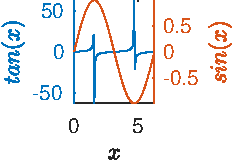
\includegraphics{../matlab/fig/examples/tansin-with-ffsp.pdf}
			\subcaption{A simple subcaption for this plot.}
		\end{subfigure}
		\hfil
		\begin{subfigure}[b]{\fourfig\textwidth} 
			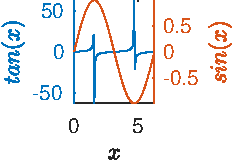
\includegraphics{../matlab/fig/examples/tansin-with-ffsp.pdf}
			\subcaption{A simple subcaption for this plot.}
		\end{subfigure}
		\hfil
		\begin{subfigure}[b]{\fourfig\textwidth} 
			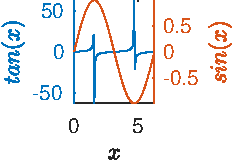
\includegraphics{../matlab/fig/examples/tansin-with-ffsp.pdf}
			\subcaption{A simple subcaption for this plot.}
		\end{subfigure}
		\hfil
		\begin{subfigure}[b]{\fourfig\textwidth} 
			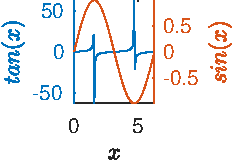
\includegraphics{../matlab/fig/examples/tansin-with-ffsp.pdf}
			\subcaption{A simple subcaption for this plot.}
		\end{subfigure}
		\\
		\begin{subfigure}[b]{\fourfig\textwidth} 
			% Add reference to the code that produced the figure
			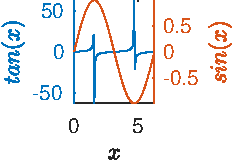
\includegraphics{../matlab/fig/examples/tansin-with-ffsp.pdf}
			\subcaption{A simple subcaption for this plot.}
		\end{subfigure}
		\hfil
		\begin{subfigure}[b]{\fourfig\textwidth} 
			% Add reference to the code that produced the figure
			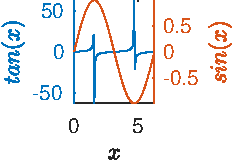
\includegraphics{../matlab/fig/examples/tansin-with-ffsp.pdf}
			\subcaption{A simple subcaption for this plot.}
		\end{subfigure}
		\hfil
		\begin{subfigure}[b]{\fourfig\textwidth} 
			% Add reference to the code that produced the figure
			\centering
			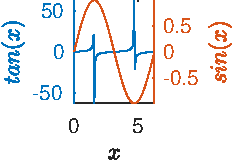
\includegraphics{../matlab/fig/examples/tansin-with-ffsp.pdf}
			\subcaption{A simple subcaption for this plot.}
		\end{subfigure}
		\hfil
		\begin{subfigure}[b]{\fourfig\textwidth} 
			% Add reference to the code that produced the figure
			\centering
			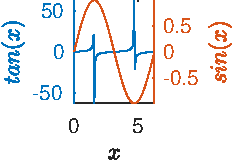
\includegraphics{../matlab/fig/examples/tansin-with-ffsp.pdf}
			\subcaption{A simple subcaption for this plot.}
		\end{subfigure}
		\\
		\begin{subfigure}[b]{\fourfig\textwidth} 
			% Add reference to the code that produced the figure
			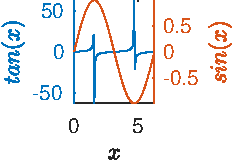
\includegraphics{../matlab/fig/examples/tansin-with-ffsp.pdf}
			\subcaption{A simple subcaption for this plot.}
		\end{subfigure}
		\hfil
		\begin{subfigure}[b]{\fourfig\textwidth} 
			% Add reference to the code that produced the figure
			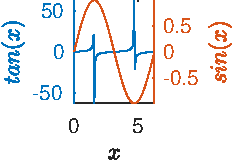
\includegraphics{../matlab/fig/examples/tansin-with-ffsp.pdf}
			\subcaption{A simple subcaption for this plot.}
		\end{subfigure}
		\hfil
		\begin{subfigure}[b]{\fourfig\textwidth} 
			% Add reference to the code that produced the figure
			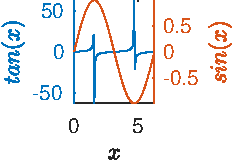
\includegraphics{../matlab/fig/examples/tansin-with-ffsp.pdf}
			\subcaption{A simple subcaption for this plot.}
		\end{subfigure}
		\hfil
		\begin{subfigure}[b]{\fourfig\textwidth} 
			% Add reference to the code that produced the figure
			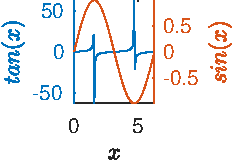
\includegraphics{../matlab/fig/examples/tansin-with-ffsp.pdf}
			\subcaption{A simple subcaption for this plot.}
		\end{subfigure}
		\\
		\begin{subfigure}[b]{\fourfig\textwidth} 
			% Add reference to the code that produced the figure
			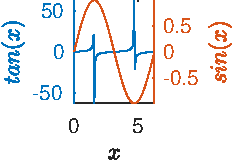
\includegraphics{../matlab/fig/examples/tansin-with-ffsp.pdf}
			\subcaption{A simple subcaption for this plot.}
		\end{subfigure}
		\hfil
		\begin{subfigure}[b]{\fourfig\textwidth} 
			% Add reference to the code that produced the figure
			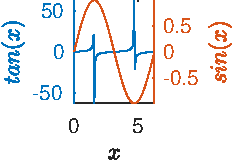
\includegraphics{../matlab/fig/examples/tansin-with-ffsp.pdf}
			\subcaption{A simple subcaption for this plot.}
		\end{subfigure}
		\hfil
		\begin{subfigure}[b]{\fourfig\textwidth} 
			% Add reference to the code that produced the figure
			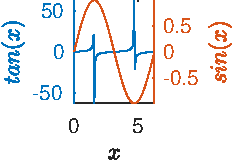
\includegraphics{../matlab/fig/examples/tansin-with-ffsp.pdf}
			\subcaption{A simple subcaption for this plot.}
		\end{subfigure}
		\hfil
		\begin{subfigure}[b]{\fourfig\textwidth} 
			% Add reference to the code that produced the figure
			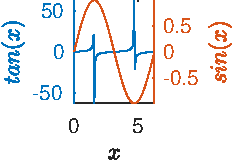
\includegraphics{../matlab/fig/examples/tansin-with-ffsp.pdf}
			\subcaption{A simple subcaption for this plot.}
		\end{subfigure}
		\caption{Two trigonometric functions in a \num{4}-by-\num{4} grid layout. \label{fig:4-by-4}}
	\end{figure}